\documentclass[1p]{elsarticle_modified}
%\bibliographystyle{elsarticle-num}

%\usepackage[colorlinks]{hyperref}
%\usepackage{abbrmath_seonhwa} %\Abb, \Ascr, \Acal ,\Abf, \Afrak
\usepackage{amsfonts}
\usepackage{amssymb}
\usepackage{amsmath}
\usepackage{amsthm}
\usepackage{scalefnt}
\usepackage{amsbsy}
\usepackage{kotex}
\usepackage{caption}
\usepackage{subfig}
\usepackage{color}
\usepackage{graphicx}
\usepackage{xcolor} %% white, black, red, green, blue, cyan, magenta, yellow
\usepackage{float}
\usepackage{setspace}
\usepackage{hyperref}

\usepackage{tikz}
\usetikzlibrary{arrows}

\usepackage{multirow}
\usepackage{array} % fixed length table
\usepackage{hhline}

%%%%%%%%%%%%%%%%%%%%%
\makeatletter
\renewcommand*\env@matrix[1][\arraystretch]{%
	\edef\arraystretch{#1}%
	\hskip -\arraycolsep
	\let\@ifnextchar\new@ifnextchar
	\array{*\c@MaxMatrixCols c}}
\makeatother %https://tex.stackexchange.com/questions/14071/how-can-i-increase-the-line-spacing-in-a-matrix
%%%%%%%%%%%%%%%

\usepackage[normalem]{ulem}

\newcommand{\msout}[1]{\ifmmode\text{\sout{\ensuremath{#1}}}\else\sout{#1}\fi}
%SOURCE: \msout is \stkout macro in https://tex.stackexchange.com/questions/20609/strikeout-in-math-mode

\newcommand{\cancel}[1]{
	\ifmmode
	{\color{red}\msout{#1}}
	\else
	{\color{red}\sout{#1}}
	\fi
}

\newcommand{\add}[1]{
	{\color{blue}\uwave{#1}}
}

\newcommand{\replace}[2]{
	\ifmmode
	{\color{red}\msout{#1}}{\color{blue}\uwave{#2}}
	\else
	{\color{red}\sout{#1}}{\color{blue}\uwave{#2}}
	\fi
}

\newcommand{\Sol}{\mathcal{S}} %segment
\newcommand{\D}{D} %diagram
\newcommand{\A}{\mathcal{A}} %arc


%%%%%%%%%%%%%%%%%%%%%%%%%%%%%5 test

\def\sl{\operatorname{\textup{SL}}(2,\Cbb)}
\def\psl{\operatorname{\textup{PSL}}(2,\Cbb)}
\def\quan{\mkern 1mu \triangleright \mkern 1mu}

\theoremstyle{definition}
\newtheorem{thm}{Theorem}[section]
\newtheorem{prop}[thm]{Proposition}
\newtheorem{lem}[thm]{Lemma}
\newtheorem{ques}[thm]{Question}
\newtheorem{cor}[thm]{Corollary}
\newtheorem{defn}[thm]{Definition}
\newtheorem{exam}[thm]{Example}
\newtheorem{rmk}[thm]{Remark}
\newtheorem{alg}[thm]{Algorithm}

\newcommand{\I}{\sqrt{-1}}
\begin{document}

%\begin{frontmatter}
%
%\title{Boundary parabolic representations of knots up to 8 crossings}
%
%%% Group authors per affiliation:
%\author{Yunhi Cho} 
%\address{Department of Mathematics, University of Seoul, Seoul, Korea}
%\ead{yhcho@uos.ac.kr}
%
%
%\author{Seonhwa Kim} %\fnref{s_kim}}
%\address{Center for Geometry and Physics, Institute for Basic Science, Pohang, 37673, Korea}
%\ead{ryeona17@ibs.re.kr}
%
%\author{Hyuk Kim}
%\address{Department of Mathematical Sciences, Seoul National University, Seoul 08826, Korea}
%\ead{hyukkim@snu.ac.kr}
%
%\author{Seokbeom Yoon}
%\address{Department of Mathematical Sciences, Seoul National University, Seoul, 08826,  Korea}
%\ead{sbyoon15@snu.ac.kr}
%
%\begin{abstract}
%We find all boundary parabolic representation of knots up to 8 crossings.
%
%\end{abstract}
%\begin{keyword}
%    \MSC[2010] 57M25 
%\end{keyword}
%
%\end{frontmatter}

%\linenumbers
%\tableofcontents
%
\newcommand\colored[1]{\textcolor{white}{\rule[-0.35ex]{0.8em}{1.4ex}}\kern-0.8em\color{red} #1}%
%\newcommand\colored[1]{\textcolor{white}{ #1}\kern-2.17ex	\textcolor{white}{ #1}\kern-1.81ex	\textcolor{white}{ #1}\kern-2.15ex\color{red}#1	}

{\Large $\underline{9_{26}~(K9a_{15})}$}

\setlength{\tabcolsep}{10pt}
\renewcommand{\arraystretch}{1.6}
\vspace{1cm}\begin{tabular}{m{100pt}>{\centering\arraybackslash}m{274pt}}
\multirow{5}{120pt}{
	\centering
	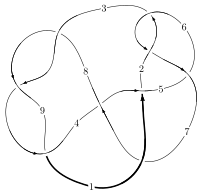
\includegraphics[width=112pt]{../../../GIT/diagram.site/Diagrams/png/61_9_26.png}\\
\ \ \ A knot diagram\footnotemark}&
\allowdisplaybreaks
\textbf{Linearized knot diagam} \\
\cline{2-2}
 &
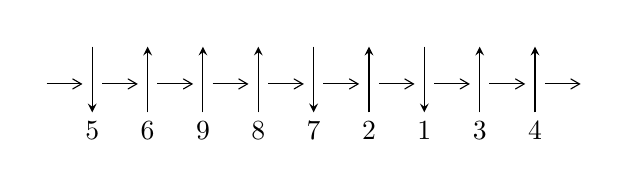
\begin{tikzpicture}[x=20pt, y=17pt]
	% nodes
	\node (C0) at (0, 0) {};
	\node (C1) at (1, 0) {};
	\node (C1U) at (1, +1) {};
	\node (C1D) at (1, -1) {5};

	\node (C2) at (2, 0) {};
	\node (C2U) at (2, +1) {};
	\node (C2D) at (2, -1) {6};

	\node (C3) at (3, 0) {};
	\node (C3U) at (3, +1) {};
	\node (C3D) at (3, -1) {9};

	\node (C4) at (4, 0) {};
	\node (C4U) at (4, +1) {};
	\node (C4D) at (4, -1) {8};

	\node (C5) at (5, 0) {};
	\node (C5U) at (5, +1) {};
	\node (C5D) at (5, -1) {7};

	\node (C6) at (6, 0) {};
	\node (C6U) at (6, +1) {};
	\node (C6D) at (6, -1) {2};

	\node (C7) at (7, 0) {};
	\node (C7U) at (7, +1) {};
	\node (C7D) at (7, -1) {1};

	\node (C8) at (8, 0) {};
	\node (C8U) at (8, +1) {};
	\node (C8D) at (8, -1) {3};

	\node (C9) at (9, 0) {};
	\node (C9U) at (9, +1) {};
	\node (C9D) at (9, -1) {4};
	\node (C10) at (10, 0) {};

	% arrows
	\draw[->,>={angle 60}]
	(C0) edge (C1) (C1) edge (C2) (C2) edge (C3) (C3) edge (C4) (C4) edge (C5) (C5) edge (C6) (C6) edge (C7) (C7) edge (C8) (C8) edge (C9) (C9) edge (C10) ;	\draw[->,>=stealth]
	(C1U) edge (C1D) (C2D) edge (C2U) (C3D) edge (C3U) (C4D) edge (C4U) (C5U) edge (C5D) (C6D) edge (C6U) (C7U) edge (C7D) (C8D) edge (C8U) (C9D) edge (C9U) ;
	\end{tikzpicture} \\
\hhline{~~} \\& 
\textbf{Solving Sequence} \\ \cline{2-2} 
 &
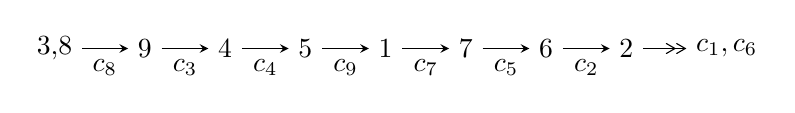
\begin{tikzpicture}[x=29pt, y=7pt]
	% node
	\node (A0) at (-1/8, 0) {3,8};
	\node (A1) at (1, 0) {9};
	\node (A2) at (2, 0) {4};
	\node (A3) at (3, 0) {5};
	\node (A4) at (4, 0) {1};
	\node (A5) at (5, 0) {7};
	\node (A6) at (6, 0) {6};
	\node (A7) at (7, 0) {2};
	\node (C1) at (1/2, -1) {$c_{8}$};
	\node (C2) at (3/2, -1) {$c_{3}$};
	\node (C3) at (5/2, -1) {$c_{4}$};
	\node (C4) at (7/2, -1) {$c_{9}$};
	\node (C5) at (9/2, -1) {$c_{7}$};
	\node (C6) at (11/2, -1) {$c_{5}$};
	\node (C7) at (13/2, -1) {$c_{2}$};
	\node (A8) at (33/4, 0) {$c_{1},c_{6}$};

	% edge
	\draw[->,>=stealth]	
	(A0) edge (A1) (A1) edge (A2) (A2) edge (A3) (A3) edge (A4) (A4) edge (A5) (A5) edge (A6) (A6) edge (A7) ;
	\draw[->>,>={angle 60}]	
	(A7) edge (A8);
\end{tikzpicture} \\ 

\end{tabular} \\

\footnotetext{
The image of knot diagram is generated by the software ``\textbf{Draw programme}" developed by Andrew Bartholomew(\url{http://www.layer8.co.uk/maths/draw/index.htm\#Running-draw}), where we modified some parts for our purpose(\url{https://github.com/CATsTAILs/LinksPainter}).
}\phantom \\ \newline 
\centering \textbf{Ideals for irreducible components\footnotemark of $X_{\text{par}}$} 
 
\begin{align*}
I^u_{1}&=\langle 
u^{23}+u^{22}+\cdots-2 u^3+1\rangle \\
\\
\end{align*}
\raggedright * 1 irreducible components of $\dim_{\mathbb{C}}=0$, with total 23 representations.\\
\footnotetext{All coefficients of polynomials are rational numbers. But the coefficients are sometimes approximated in decimal forms when there is not enough margin.}
\newpage
\renewcommand{\arraystretch}{1}
\centering \section*{I. $I^u_{1}= \langle u^{23}+u^{22}+\cdots-2 u^3+1 \rangle$}
\flushleft \textbf{(i) Arc colorings}\\
\begin{tabular}{m{7pt} m{180pt} m{7pt} m{180pt} }
\flushright $a_{3}=$&$\begin{pmatrix}0\\u\end{pmatrix}$ \\
\flushright $a_{8}=$&$\begin{pmatrix}1\\0\end{pmatrix}$ \\
\flushright $a_{9}=$&$\begin{pmatrix}1\\- u^2\end{pmatrix}$ \\
\flushright $a_{4}=$&$\begin{pmatrix}u\\- u^3+u\end{pmatrix}$ \\
\flushright $a_{5}=$&$\begin{pmatrix}- u^3+2 u\\- u^3+u\end{pmatrix}$ \\
\flushright $a_{1}=$&$\begin{pmatrix}- u^2+1\\u^4-2 u^2\end{pmatrix}$ \\
\flushright $a_{7}=$&$\begin{pmatrix}u^6-3 u^4+2 u^2+1\\- u^8+4 u^6-4 u^4\end{pmatrix}$ \\
\flushright $a_{6}=$&$\begin{pmatrix}u^{17}-8 u^{15}+25 u^{13}-36 u^{11}+19 u^9+4 u^7-2 u^5-4 u^3+u\\- u^{19}+9 u^{17}-32 u^{15}+55 u^{13}-43 u^{11}+9 u^9+4 u^5- u^3+u\end{pmatrix}$ \\
\flushright $a_{2}=$&$\begin{pmatrix}- u^{10}+5 u^8-8 u^6+3 u^4+u^2+1\\- u^{10}+4 u^8-5 u^6+2 u^4- u^2\end{pmatrix}$\\ \flushright $a_{2}=$&$\begin{pmatrix}- u^{10}+5 u^8-8 u^6+3 u^4+u^2+1\\- u^{10}+4 u^8-5 u^6+2 u^4- u^2\end{pmatrix}$\\&\end{tabular}
\flushleft \textbf{(ii) Obstruction class $= -1$}\\~\\
\flushleft \textbf{(iii) Cusp Shapes $= -4 u^{20}+36 u^{18}-4 u^{17}-132 u^{16}+32 u^{15}+244 u^{14}-100 u^{13}-220 u^{12}+144 u^{11}+60 u^{10}-80 u^9+24 u^8+4 u^6-12 u^5-8 u^4+20 u^3-4 u^2+2$}\\~\\
\newpage\renewcommand{\arraystretch}{1}
\flushleft \textbf{(iv) u-Polynomials at the component}\newline \\
\begin{tabular}{m{50pt}|m{274pt}}
Crossings & \hspace{64pt}u-Polynomials at each crossing \\
\hline $$\begin{aligned}c_{1}\end{aligned}$$&$\begin{aligned}
&u^{23}+u^{22}+\cdots-8 u-5
\end{aligned}$\\
\hline $$\begin{aligned}c_{2},c_{6}\end{aligned}$$&$\begin{aligned}
&u^{23}- u^{22}+\cdots+2 u-1
\end{aligned}$\\
\hline $$\begin{aligned}c_{3},c_{8},c_{9}\end{aligned}$$&$\begin{aligned}
&u^{23}- u^{22}+\cdots-2 u^3-1
\end{aligned}$\\
\hline $$\begin{aligned}c_{4}\end{aligned}$$&$\begin{aligned}
&u^{23}+3 u^{22}+\cdots+4 u+1
\end{aligned}$\\
\hline $$\begin{aligned}c_{5}\end{aligned}$$&$\begin{aligned}
&u^{23}+11 u^{22}+\cdots-2 u^2-1
\end{aligned}$\\
\hline $$\begin{aligned}c_{7}\end{aligned}$$&$\begin{aligned}
&u^{23}-5 u^{22}+\cdots+32 u-7
\end{aligned}$\\
\hline
\end{tabular}\\~\\
\newpage\renewcommand{\arraystretch}{1}
\flushleft \textbf{(v) Riley Polynomials at the component}\newline \\
\begin{tabular}{m{50pt}|m{274pt}}
Crossings & \hspace{64pt}Riley Polynomials at each crossing \\
\hline $$\begin{aligned}c_{1}\end{aligned}$$&$\begin{aligned}
&y^{23}-5 y^{22}+\cdots+264 y-25
\end{aligned}$\\
\hline $$\begin{aligned}c_{2},c_{6}\end{aligned}$$&$\begin{aligned}
&y^{23}+11 y^{22}+\cdots-2 y^2-1
\end{aligned}$\\
\hline $$\begin{aligned}c_{3},c_{8},c_{9}\end{aligned}$$&$\begin{aligned}
&y^{23}-21 y^{22}+\cdots-6 y^2-1
\end{aligned}$\\
\hline $$\begin{aligned}c_{4}\end{aligned}$$&$\begin{aligned}
&y^{23}- y^{22}+\cdots+4 y-1
\end{aligned}$\\
\hline $$\begin{aligned}c_{5}\end{aligned}$$&$\begin{aligned}
&y^{23}+3 y^{22}+\cdots-4 y-1
\end{aligned}$\\
\hline $$\begin{aligned}c_{7}\end{aligned}$$&$\begin{aligned}
&y^{23}+7 y^{22}+\cdots-404 y-49
\end{aligned}$\\
\hline
\end{tabular}\\~\\
\newpage\flushleft \textbf{(vi) Complex Volumes and Cusp Shapes}
$$\begin{array}{c|c|c}  
\text{Solutions to }I^u_{1}& \I (\text{vol} + \sqrt{-1}CS) & \text{Cusp shape}\\
 \hline 
\begin{aligned}
u &= \phantom{-}1.070060 + 0.182203 I\end{aligned}
 & -1.02537 + 3.60580 I & \phantom{-}1.11445 - 4.48858 I \\ \hline\begin{aligned}
u &= \phantom{-}1.070060 - 0.182203 I\end{aligned}
 & -1.02537 - 3.60580 I & \phantom{-}1.11445 + 4.48858 I \\ \hline\begin{aligned}
u &= -1.15018\phantom{ +0.000000I}\end{aligned}
 & \phantom{-}1.95316\phantom{ +0.000000I} & \phantom{-}5.52610\phantom{ +0.000000I} \\ \hline\begin{aligned}
u &= \phantom{-}0.285113 + 0.703745 I\end{aligned}
 & -2.00141 + 7.02777 I & \phantom{-}0.43599 - 7.34039 I \\ \hline\begin{aligned}
u &= \phantom{-}0.285113 - 0.703745 I\end{aligned}
 & -2.00141 - 7.02777 I & \phantom{-}0.43599 + 7.34039 I \\ \hline\begin{aligned}
u &= \phantom{-}0.625021 + 0.336059 I\end{aligned}
 & -0.61995 - 3.26242 I & \phantom{-}3.19624 + 2.26815 I \\ \hline\begin{aligned}
u &= \phantom{-}0.625021 - 0.336059 I\end{aligned}
 & -0.61995 + 3.26242 I & \phantom{-}3.19624 - 2.26815 I \\ \hline\begin{aligned}
u &= -0.284234 + 0.630366 I\end{aligned}
 & \phantom{-}0.22041 - 2.29224 I & \phantom{-}3.82667 + 3.81893 I \\ \hline\begin{aligned}
u &= -0.284234 - 0.630366 I\end{aligned}
 & \phantom{-}0.22041 + 2.29224 I & \phantom{-}3.82667 - 3.81893 I \\ \hline\begin{aligned}
u &= \phantom{-}0.143415 + 0.670993 I\end{aligned}
 & -3.74248 - 0.30335 I & -3.41146 - 0.40480 I \\ \hline\begin{aligned}
u &= \phantom{-}0.143415 - 0.670993 I\end{aligned}
 & -3.74248 + 0.30335 I & -3.41146 + 0.40480 I \\ \hline\begin{aligned}
u &= -1.347540 + 0.251864 I\end{aligned}
 & \phantom{-}0.95696 - 3.02476 I & \phantom{-}1.87787 + 2.21609 I \\ \hline\begin{aligned}
u &= -1.347540 - 0.251864 I\end{aligned}
 & \phantom{-}0.95696 + 3.02476 I & \phantom{-}1.87787 - 2.21609 I \\ \hline\begin{aligned}
u &= -0.405548 + 0.414027 I\end{aligned}
 & \phantom{-}1.014040 - 0.946726 I & \phantom{-}6.43633 + 4.33310 I \\ \hline\begin{aligned}
u &= -0.405548 - 0.414027 I\end{aligned}
 & \phantom{-}1.014040 + 0.946726 I & \phantom{-}6.43633 - 4.33310 I \\ \hline\begin{aligned}
u &= \phantom{-}1.41968 + 0.16903 I\end{aligned}
 & \phantom{-}6.78087 + 3.16234 I & \phantom{-}9.66460 - 3.46689 I \\ \hline\begin{aligned}
u &= \phantom{-}1.41968 - 0.16903 I\end{aligned}
 & \phantom{-}6.78087 - 3.16234 I & \phantom{-}9.66460 + 3.46689 I \\ \hline\begin{aligned}
u &= -1.42608 + 0.11950 I\end{aligned}
 & \phantom{-}5.64121 + 1.73636 I & \phantom{-}7.79313 - 2.46590 I \\ \hline\begin{aligned}
u &= -1.42608 - 0.11950 I\end{aligned}
 & \phantom{-}5.64121 - 1.73636 I & \phantom{-}7.79313 + 2.46590 I \\ \hline\begin{aligned}
u &= \phantom{-}1.41107 + 0.24900 I\end{aligned}
 & \phantom{-}5.63952 + 5.52406 I & \phantom{-}8.27222 - 3.52157 I \\ \hline\begin{aligned}
u &= \phantom{-}1.41107 - 0.24900 I\end{aligned}
 & \phantom{-}5.63952 - 5.52406 I & \phantom{-}8.27222 + 3.52157 I \\ \hline\begin{aligned}
u &= -1.41586 + 0.27635 I\end{aligned}
 & \phantom{-}3.43142 - 10.59580 I & \phantom{-}5.03092 + 7.47788 I \\ \hline\begin{aligned}
u &= -1.41586 - 0.27635 I\end{aligned}
 & \phantom{-}3.43142 + 10.59580 I & \phantom{-}5.03092 - 7.47788 I\\
 \hline 
 \end{array}$$\newpage
\newpage\renewcommand{\arraystretch}{1}
\centering \section*{ II. u-Polynomials}
\begin{tabular}{m{50pt}|m{274pt}}
Crossings & \hspace{64pt}u-Polynomials at each crossing \\
\hline $$\begin{aligned}c_{1}\end{aligned}$$&$\begin{aligned}
&u^{23}+u^{22}+\cdots-8 u-5
\end{aligned}$\\
\hline $$\begin{aligned}c_{2},c_{6}\end{aligned}$$&$\begin{aligned}
&u^{23}- u^{22}+\cdots+2 u-1
\end{aligned}$\\
\hline $$\begin{aligned}c_{3},c_{8},c_{9}\end{aligned}$$&$\begin{aligned}
&u^{23}- u^{22}+\cdots-2 u^3-1
\end{aligned}$\\
\hline $$\begin{aligned}c_{4}\end{aligned}$$&$\begin{aligned}
&u^{23}+3 u^{22}+\cdots+4 u+1
\end{aligned}$\\
\hline $$\begin{aligned}c_{5}\end{aligned}$$&$\begin{aligned}
&u^{23}+11 u^{22}+\cdots-2 u^2-1
\end{aligned}$\\
\hline $$\begin{aligned}c_{7}\end{aligned}$$&$\begin{aligned}
&u^{23}-5 u^{22}+\cdots+32 u-7
\end{aligned}$\\
\hline
\end{tabular}\newpage\renewcommand{\arraystretch}{1}
\centering \section*{ III. Riley Polynomials}
\begin{tabular}{m{50pt}|m{274pt}}
Crossings & \hspace{64pt}Riley Polynomials at each crossing \\
\hline $$\begin{aligned}c_{1}\end{aligned}$$&$\begin{aligned}
&y^{23}-5 y^{22}+\cdots+264 y-25
\end{aligned}$\\
\hline $$\begin{aligned}c_{2},c_{6}\end{aligned}$$&$\begin{aligned}
&y^{23}+11 y^{22}+\cdots-2 y^2-1
\end{aligned}$\\
\hline $$\begin{aligned}c_{3},c_{8},c_{9}\end{aligned}$$&$\begin{aligned}
&y^{23}-21 y^{22}+\cdots-6 y^2-1
\end{aligned}$\\
\hline $$\begin{aligned}c_{4}\end{aligned}$$&$\begin{aligned}
&y^{23}- y^{22}+\cdots+4 y-1
\end{aligned}$\\
\hline $$\begin{aligned}c_{5}\end{aligned}$$&$\begin{aligned}
&y^{23}+3 y^{22}+\cdots-4 y-1
\end{aligned}$\\
\hline $$\begin{aligned}c_{7}\end{aligned}$$&$\begin{aligned}
&y^{23}+7 y^{22}+\cdots-404 y-49
\end{aligned}$\\
\hline
\end{tabular}
\vskip 2pc
\end{document}